\newpage
\chapter{Additional details on Convolutional Neural Network ID}
\label{Adx2}
Additional control plots for CNN ID are shown here.

\section{Background rejection for CNN Tight and Loose WPs}
\label{Adx2:BkgRej}
The background rejection of the CNN Tight and Loose WPs is shown in Figure \ref{BkgRej}. Note that the two WPs are optimized to deliver similar background rejection as the cut-based in bin of $|\eta|$. The optimization is done in the $Z\rightarrow ll\gamma$ events, while figures shows the background rejection in the Z+jets sample. This serves as an additional validation of the CNN performance. 

\begin{figure}[ht]
    \centering
	\subfloat[][]{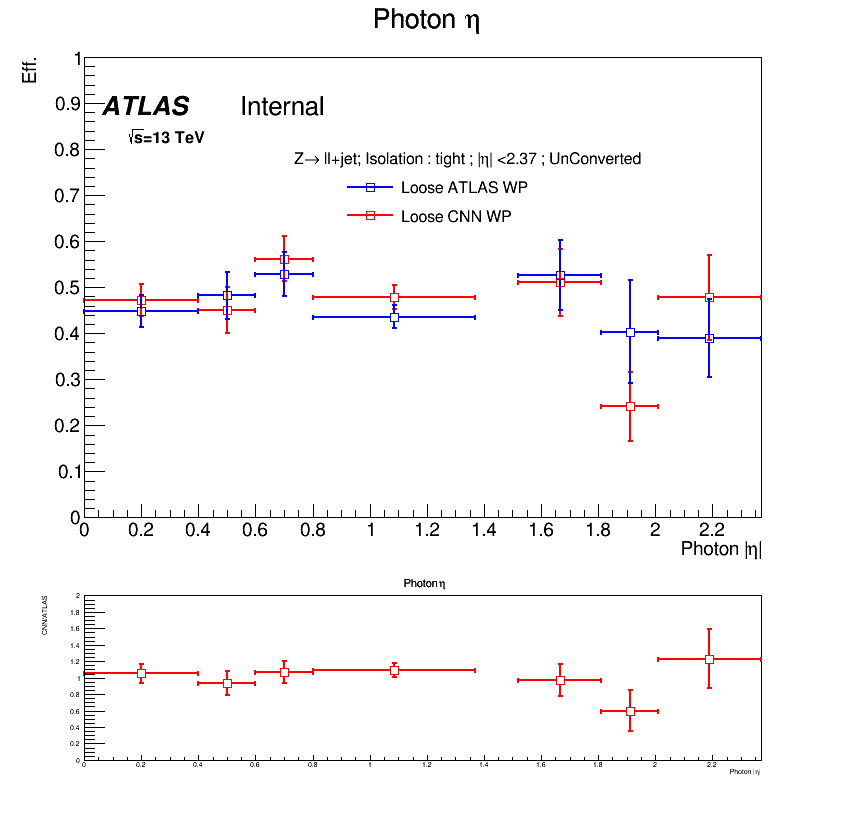
\includegraphics[width=.35\textwidth]{Adx/Adx2/Img/BackRej_ETA_UnConverted_Loose_E_Loose_E_CNN_Iso_tight.png}}
	\subfloat[][]{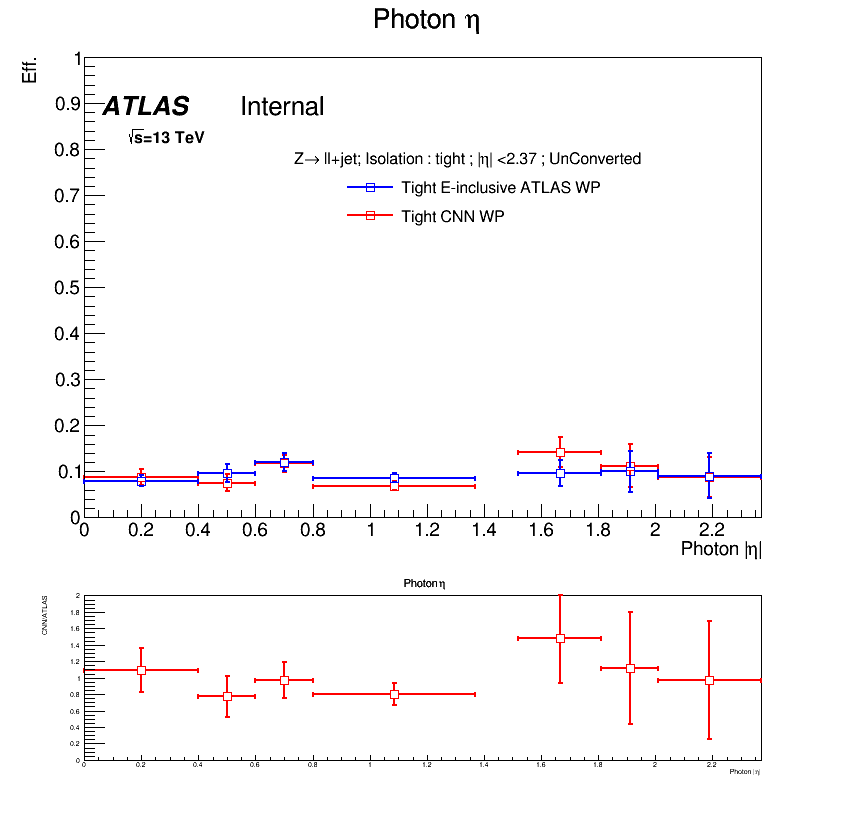
\includegraphics[width=.35\textwidth]{Adx/Adx2/Img/BackRej_ETA_UnConverted_Tight_E_inc_Tight_E_CNN_Iso_tight.png}} \\
	\subfloat[][]{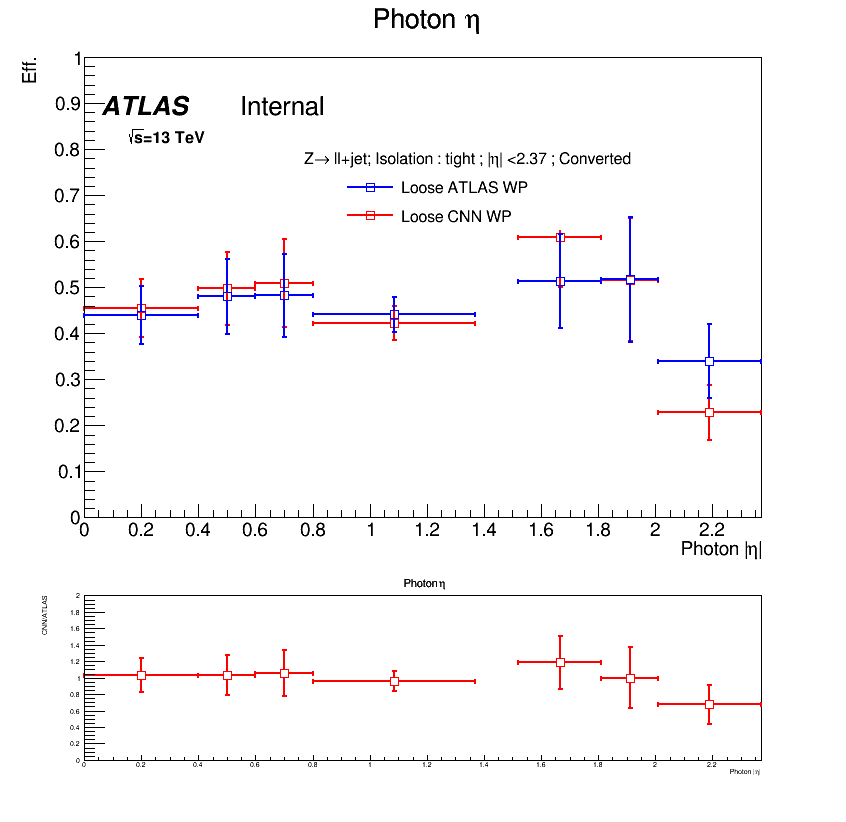
\includegraphics[width=.35\textwidth]{Adx/Adx2/Img/BackRej_ETA_Converted_Loose_E_Loose_E_CNN_Iso_tight.png}}
	\subfloat[][]{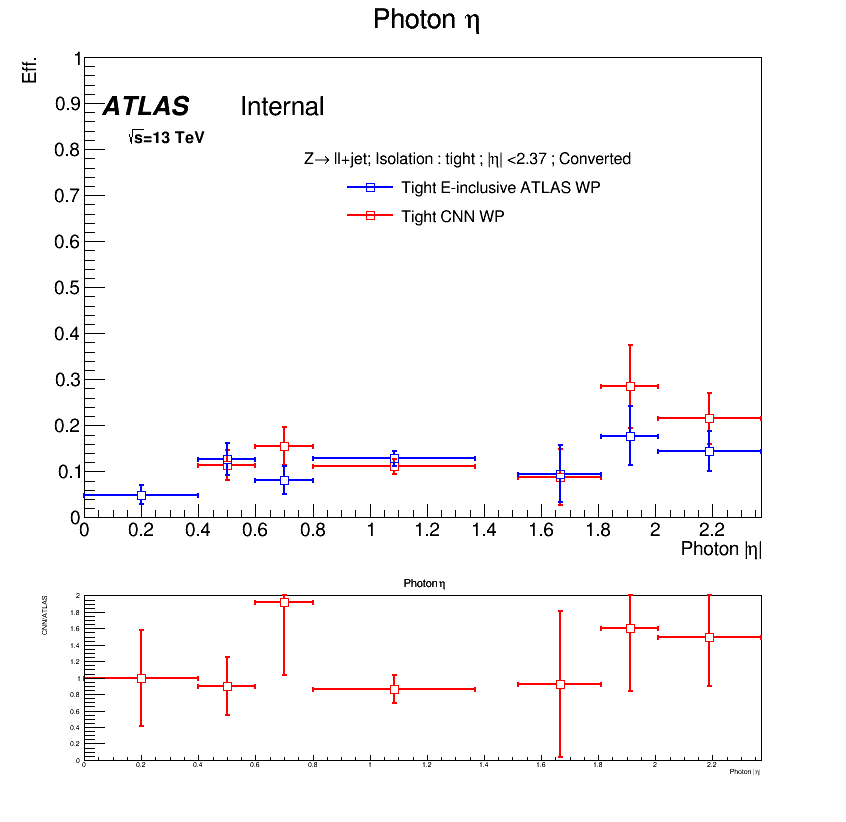
\includegraphics[width=.35\textwidth]{Adx/Adx2/Img/BackRej_ETA_Converted_Tight_E_inc_Tight_E_CNN_Iso_tight.png}}
    \caption{Background rejection of the CNN Tight (right) and Loose (left) WPs. For unconverted (top) and converted (bottom) photons in bin of $|\eta|$. The rejection is evaluated in the Z+jets sample. Red line shows the rejection for CNN and blue line shows the cut-based rejection.}
    \label{BkgRej}
\end{figure}

\section{CNN efficiency as a function of $|\eta|$}
\label{Adx2:Eff:Eta}
The CNN efficiency as a function of $|\eta|$ is shown in the following Figures \ref{Eff:Loose}, \ref{Eff:Tight:Dep} and \ref{Eff:Tight:Inc}. A comparison with the cut-based efficiencies is also shown.  

\begin{figure}[ht]
    \centering
	\subfloat[][]{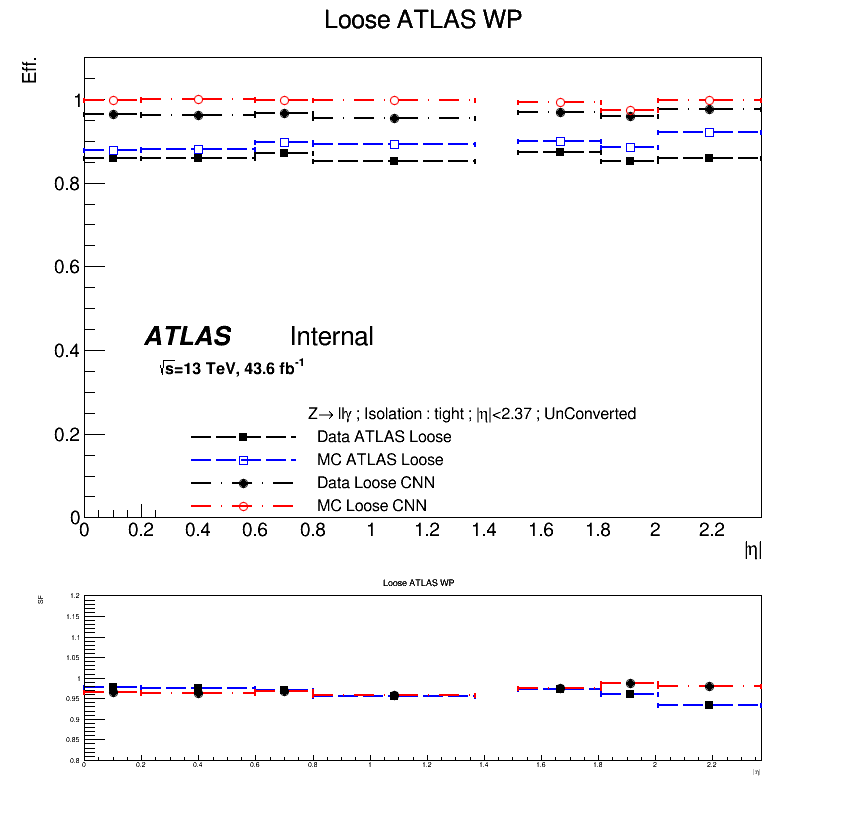
\includegraphics[width=.35\textwidth]{Adx/Adx2/Img/Loose_Wp_vs_Loose_CNN_ETA_UnConverted_Iso_tight_Wgt.png}}
	\subfloat[][]{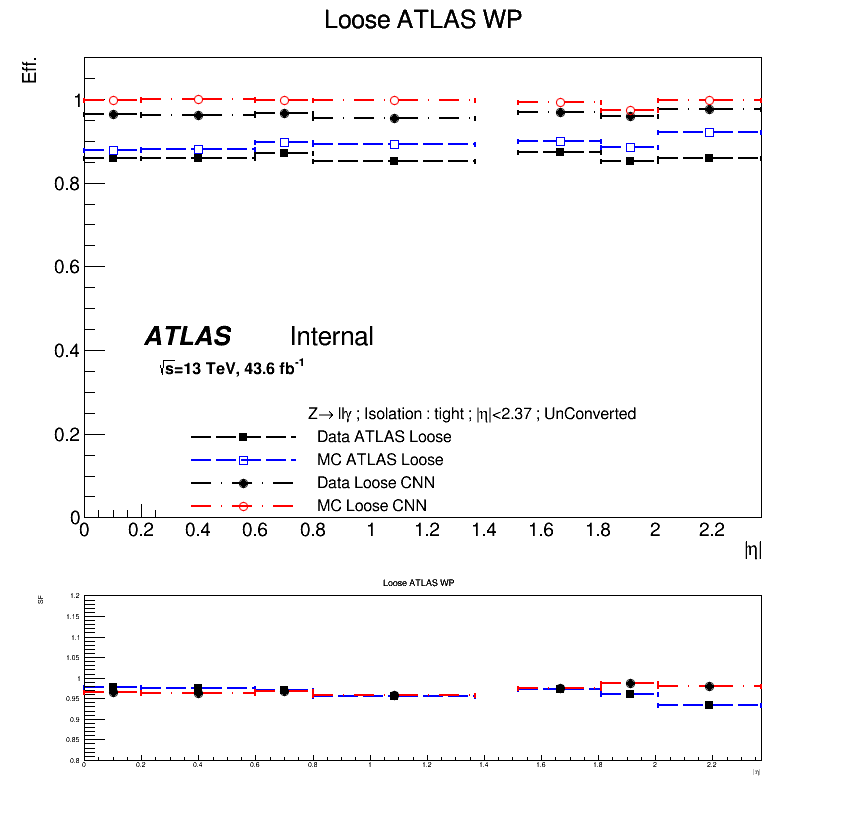
\includegraphics[width=.35\textwidth]{Adx/Adx2/Img/Loose_Wp_vs_Loose_CNN_ETA_UnConverted_Iso_tight_Wgt.png}} 
    \caption{A comparison between the CNN (red) and cut-based (blue) Loose WPs for unconverted (right)  converted (left) photons in bin of $|\eta|$. The ratio plot shows the scale factors.}
    \label{Eff:Loose}
\end{figure}

\begin{figure}[ht]
    \centering
	\subfloat[][]{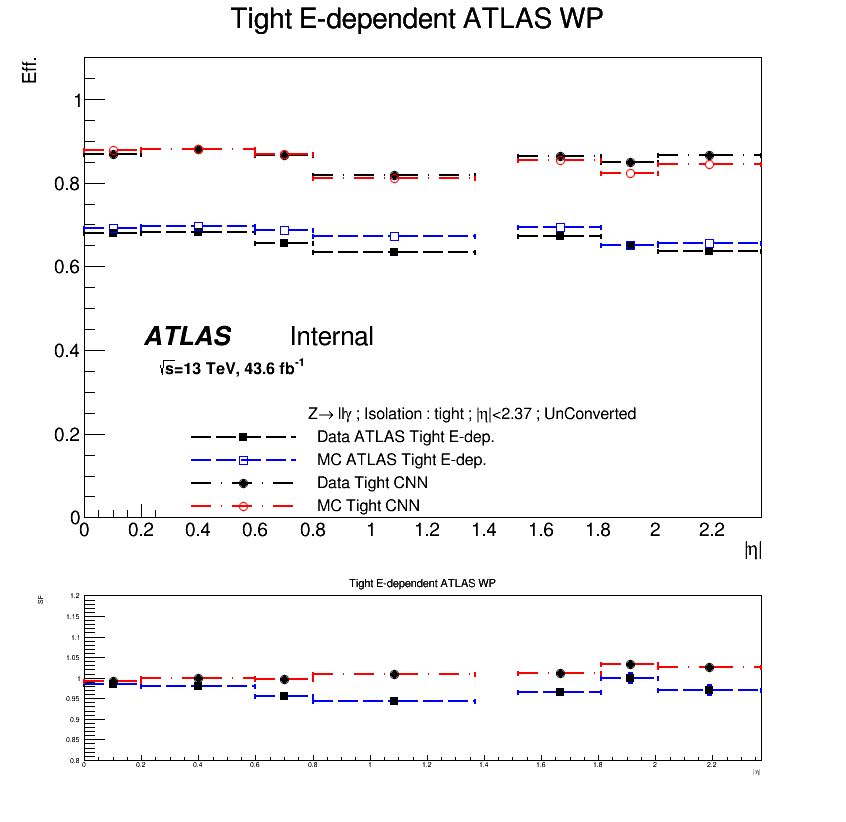
\includegraphics[width=.35\textwidth]{Adx/Adx2/Img/Tight_Dep_vs_Tight_CNN_ETA_UnConverted_Iso_tight_Wgt.png}}
	\subfloat[][]{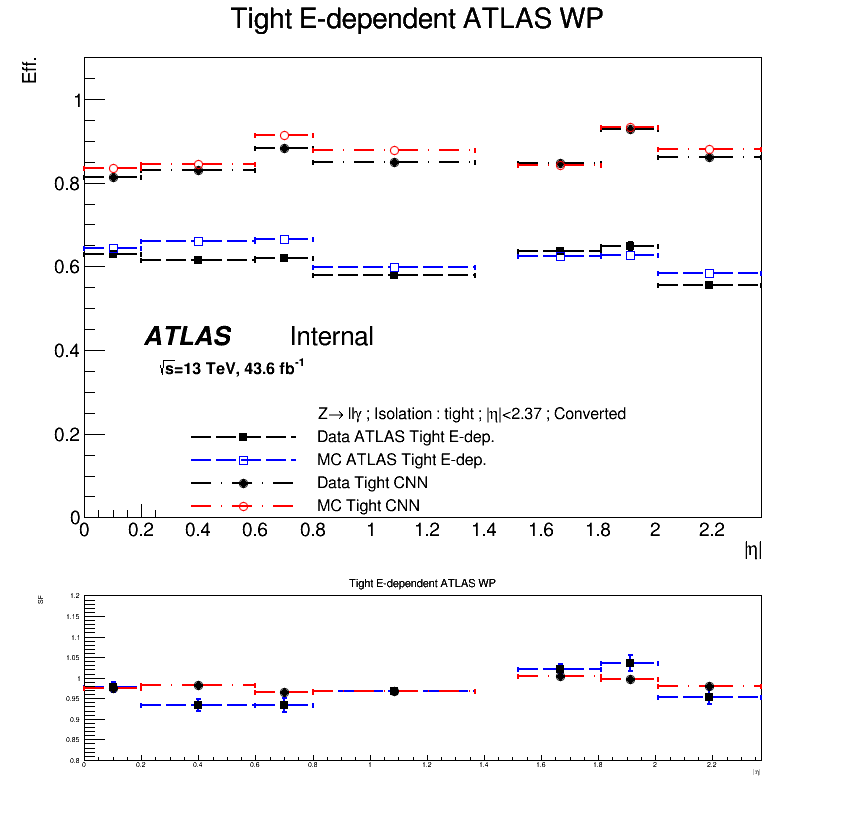
\includegraphics[width=.35\textwidth]{Adx/Adx2/Img/Tight_Dep_vs_Tight_CNN_ETA_Converted_Iso_tight_Wgt.png}} 
    \caption{A comparison between the Tight CNN (red) and Tight E-dependent cut-based  (blue) WPs for unconverted (right) converted (left) photons in bin of $|\eta|$. The ratio plot shows the scale factors.}
    \label{Eff:Tight:Dep}
\end{figure}
\begin{figure}[ht]
    \centering
	\subfloat[][]{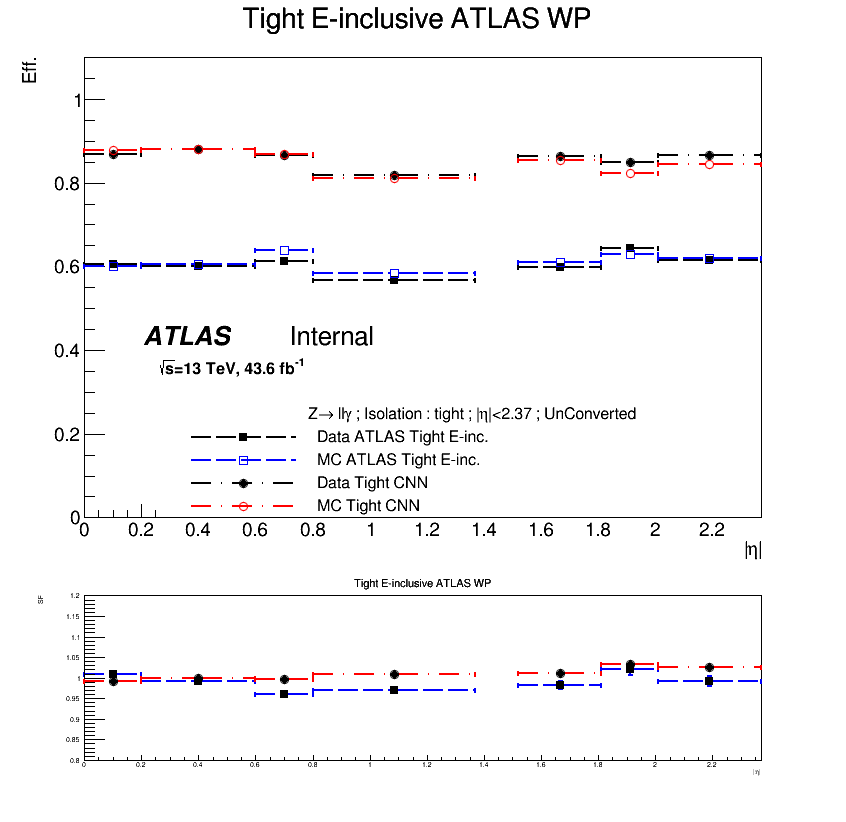
\includegraphics[width=.35\textwidth]{Adx/Adx2/Img/Tight_Inc_vs_Tight_CNN_ETA_UnConverted_Iso_tight_Wgt.png}}
	\subfloat[][]{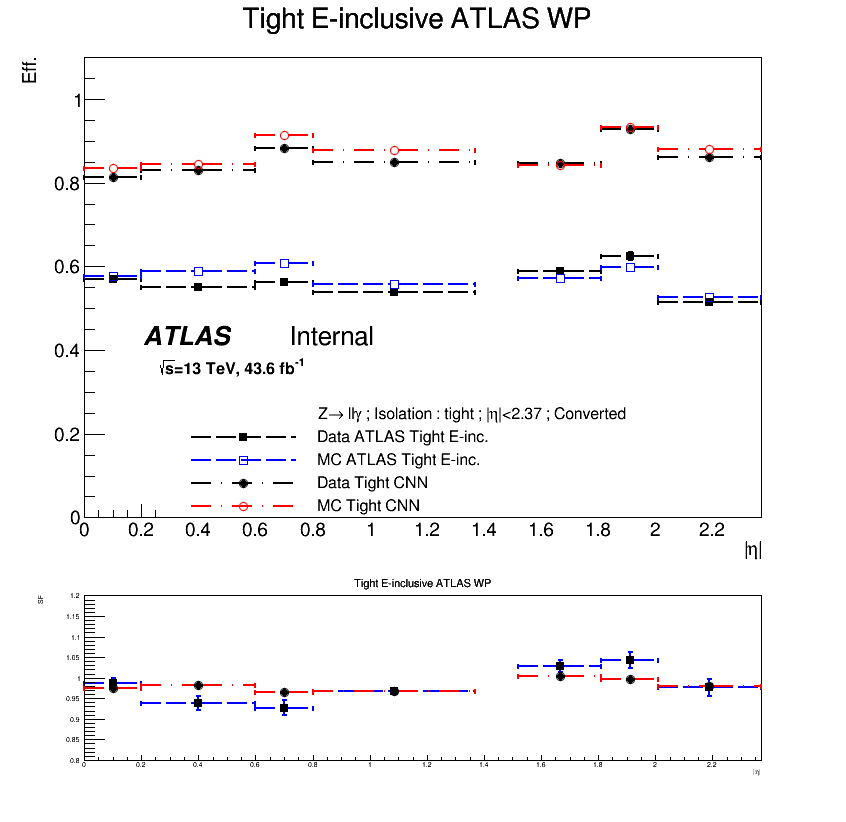
\includegraphics[width=.35\textwidth]{Adx/Adx2/Img/Tight_Inc_vs_Tight_CNN_ETA_Converted_Iso_tight_Wgt.png}} 
    \caption{A comparison between the Tight CNN (red) and Tight E-independent cut-based  (blue) WPs for unconverted (right) converted (left) photons in bin of $|\eta|$. The ratio plot shows the scale factors.}
    \label{Eff:Tight:Inc}
\end{figure}

\section{CNN efficiency in additional $|\eta|$ bins}
Figure \ref{Eff:Tight:AddBins} shows the efficiency of the CNN as evaluated using the template fit method for additional $|\eta|$ bins not provided in the main body of the thesis.
\begin{figure}[ht]
    \centering
	\subfloat[][]{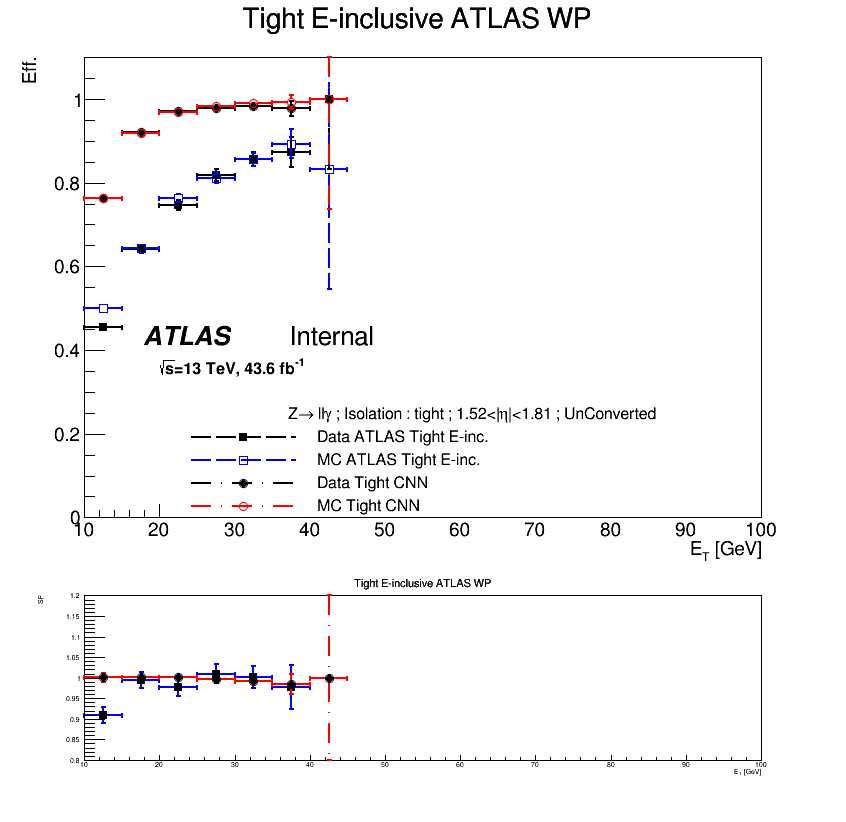
\includegraphics[width=.25\textwidth]{Adx/Adx2/Img/Tight_Inc_vs_Tight_CNN__UnConverted_Iso_tight_Wgt_ETA_Bin_5.png}}
	\subfloat[][]{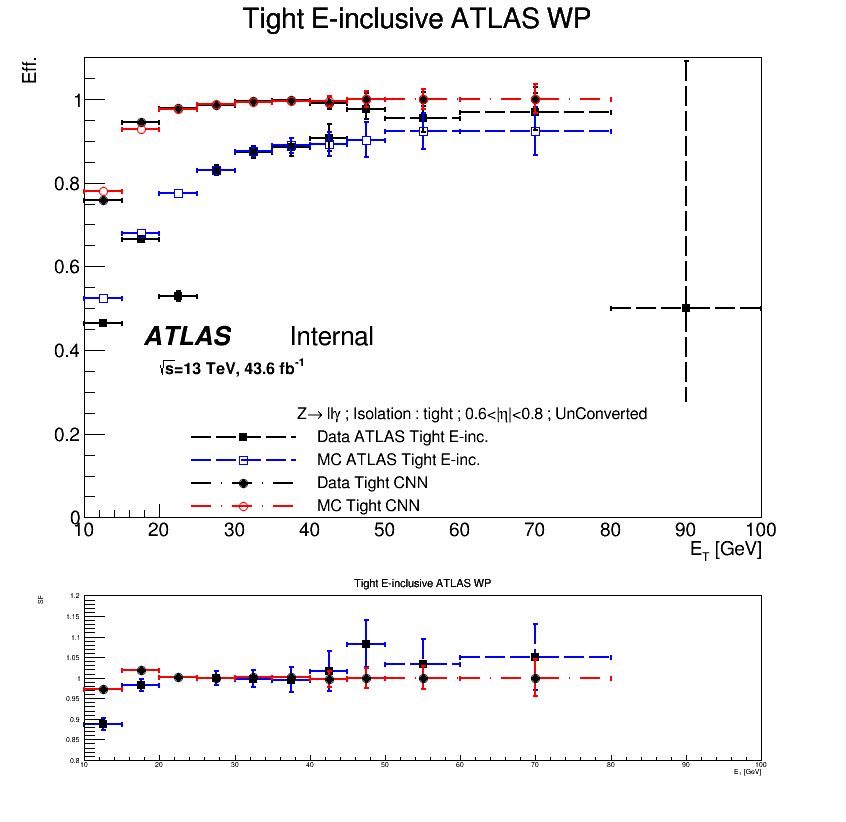
\includegraphics[width=.25\textwidth]{Adx/Adx2/Img/Tight_Inc_vs_Tight_CNN__UnConverted_Iso_tight_Wgt_ETA_Bin_6.png}}
	\subfloat[][]{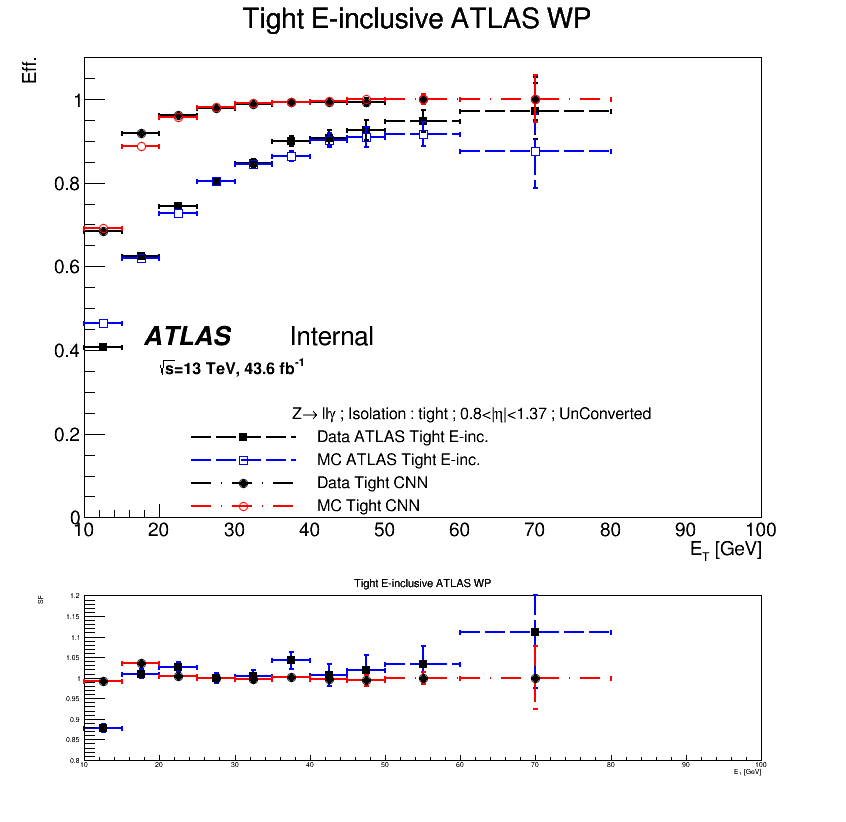
\includegraphics[width=.25\textwidth]{Adx/Adx2/Img/Tight_Inc_vs_Tight_CNN__UnConverted_Iso_tight_Wgt_ETA_Bin_7.png}}  \\
	
	\subfloat[][]{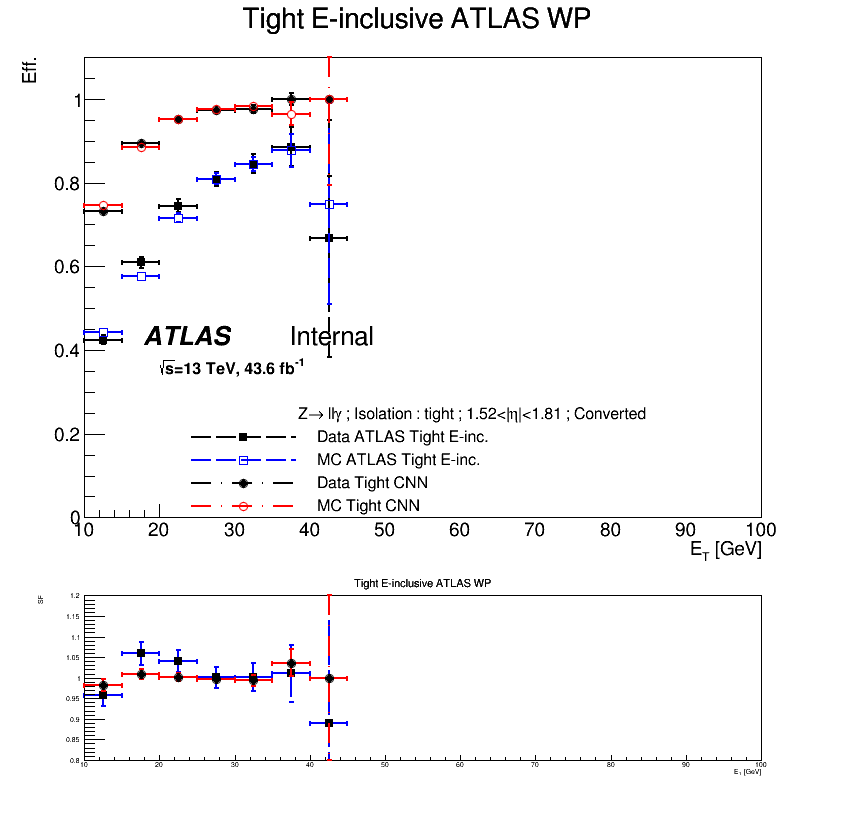
\includegraphics[width=.25\textwidth]{Adx/Adx2/Img/Tight_Inc_vs_Tight_CNN__Converted_Iso_tight_Wgt_ETA_Bin_5.png}}
	\subfloat[][]{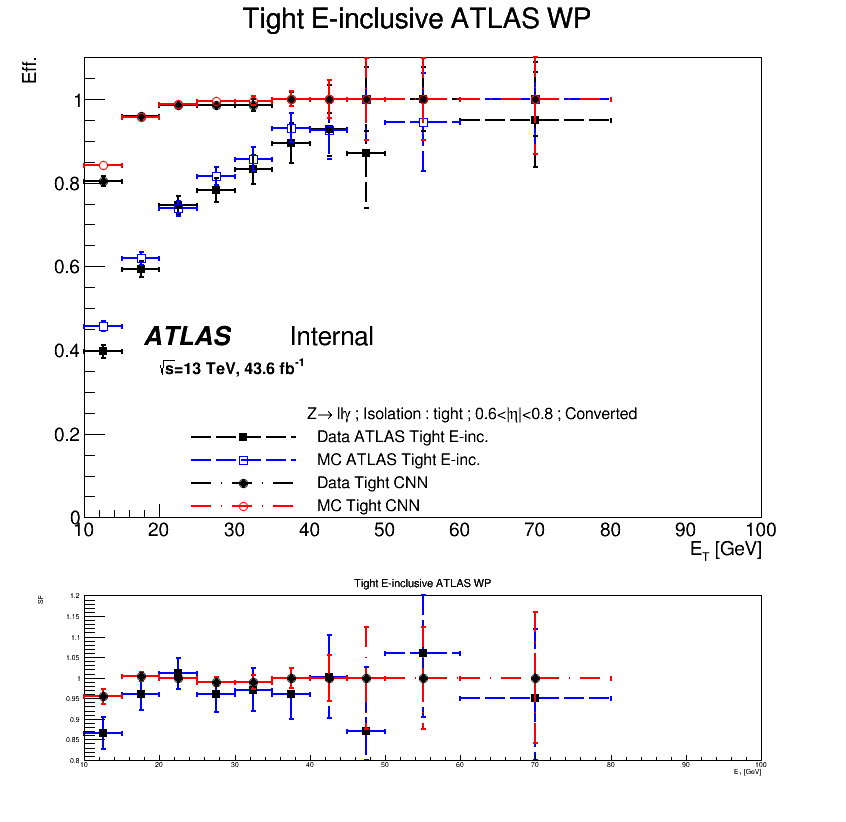
\includegraphics[width=.25\textwidth]{Adx/Adx2/Img/Tight_Inc_vs_Tight_CNN__Converted_Iso_tight_Wgt_ETA_Bin_6.png}}
	\subfloat[][]{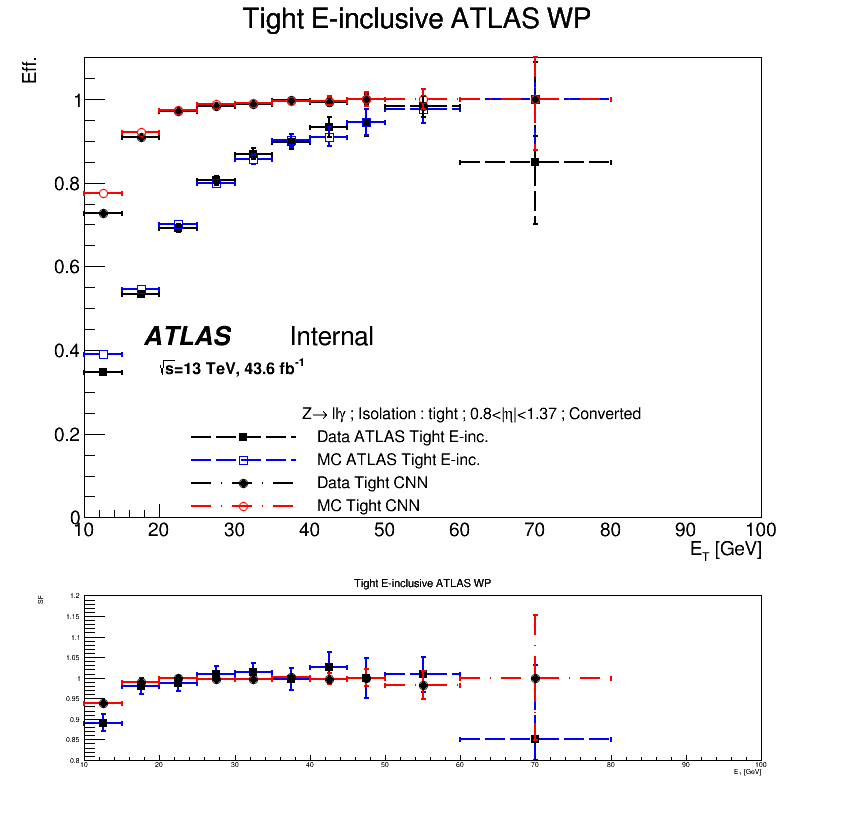
\includegraphics[width=.25\textwidth]{Adx/Adx2/Img/Tight_Inc_vs_Tight_CNN__Converted_Iso_tight_Wgt_ETA_Bin_7.png}} 
    \caption{A comparison between the Tight CNN (red) and Tight E-independent cut-based as a function of photons \eT in different bin of $|\eta|$ for unconverted (top) and converted (bottom) photons. The ratio plot shows the scale factors.}
    \label{Eff:Tight:AddBins}
\end{figure}

\section{Purity evaluation using the template fit method}
\label{Adx2:TemplateFit}
The template fit results are shown in Figures \ref{Eff:TemplateFit:UnC:Before}, \ref{Eff:TemplateFit:C:Before}, \ref{Eff:TemplateFit:UnC:After} and \ref{Eff:TemplateFit:C:After}. 

\begin{figure}[ht]
    \centering
	\subfloat[][]{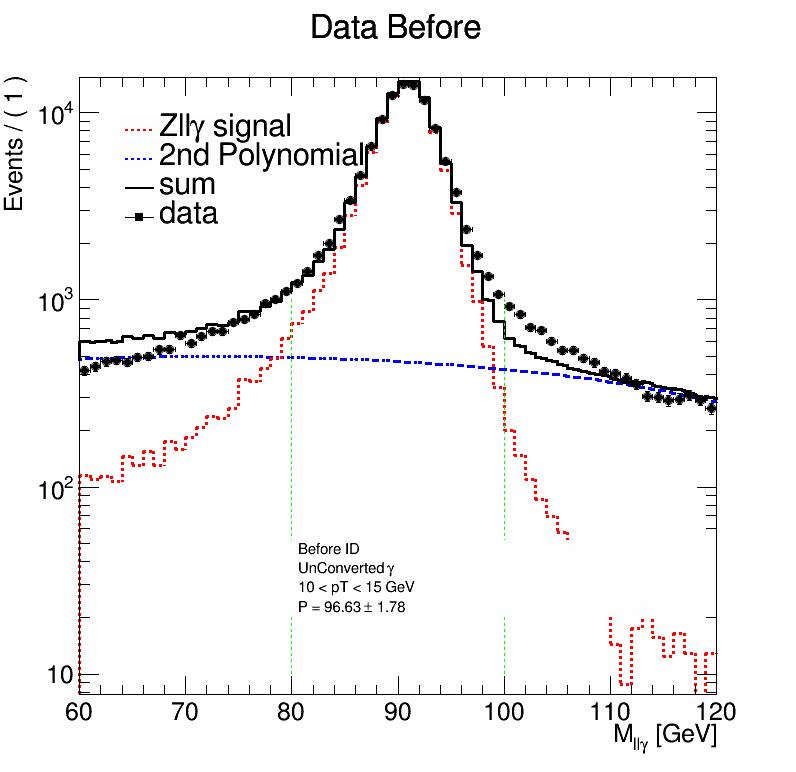
\includegraphics[width=.35\textwidth]{Adx/Adx2/Img/UnConvertedllg_Before_ID_Bin_0.png}}
	\subfloat[][]{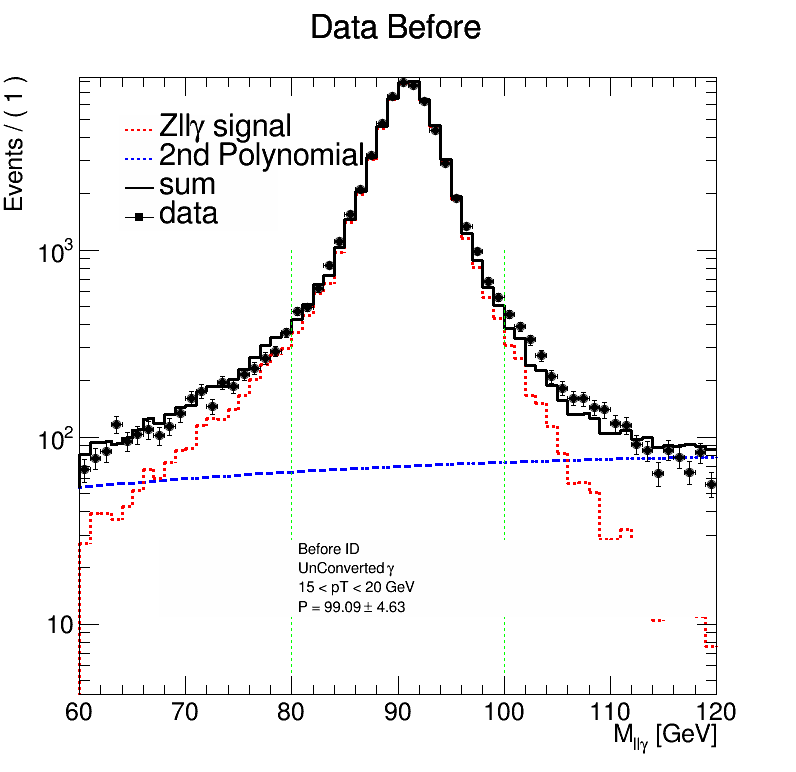
\includegraphics[width=.35\textwidth]{Adx/Adx2/Img/UnConvertedllg_Before_ID_Bin_1.png}} \\
	\subfloat[][]{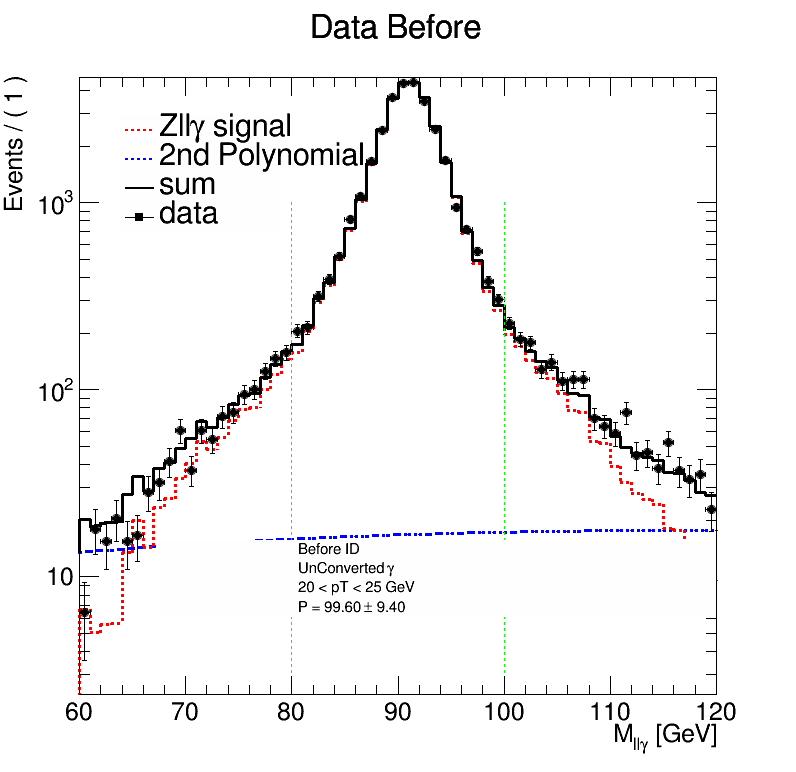
\includegraphics[width=.35\textwidth]{Adx/Adx2/Img/UnConvertedllg_Before_ID_Bin_2.png}}  
	\subfloat[][]{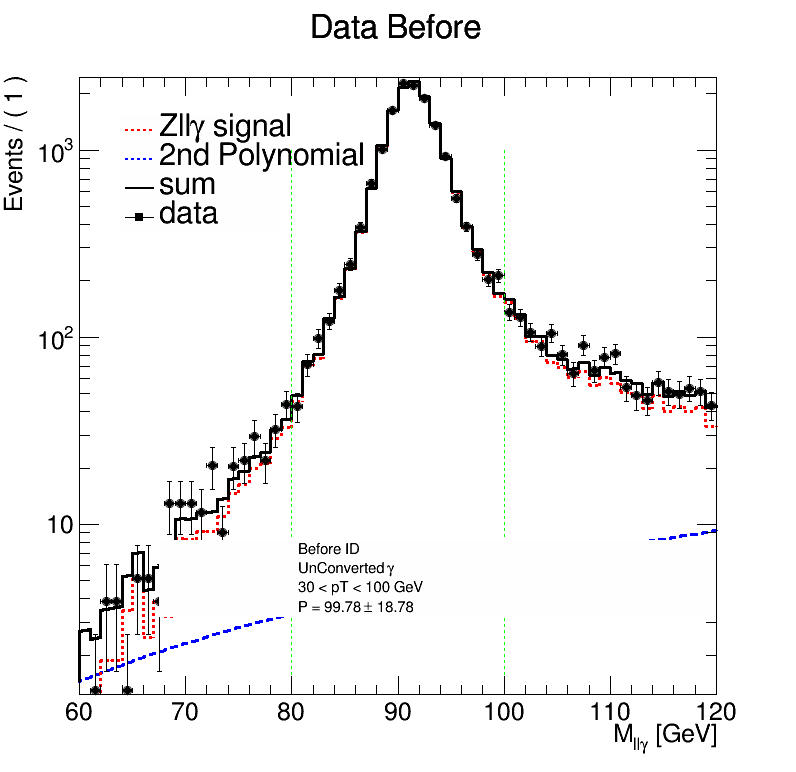
\includegraphics[width=.35\textwidth]{Adx/Adx2/Img/UnConvertedllg_Before_ID_Bin_4.png}}  
    \caption{Invariant mass ($m_{ll\gamma}$) distribution of events selected before Tight ID in data (black dots). The solid black line represents the fitting result of the data distribution with the sum of the signal (red dashed line) and the background (blue dashed line). The photons are reconstructed as unconverted.}
    \label{Eff:TemplateFit:UnC:Before}
\end{figure}

\begin{figure}[ht]
    \centering
	\subfloat[][]{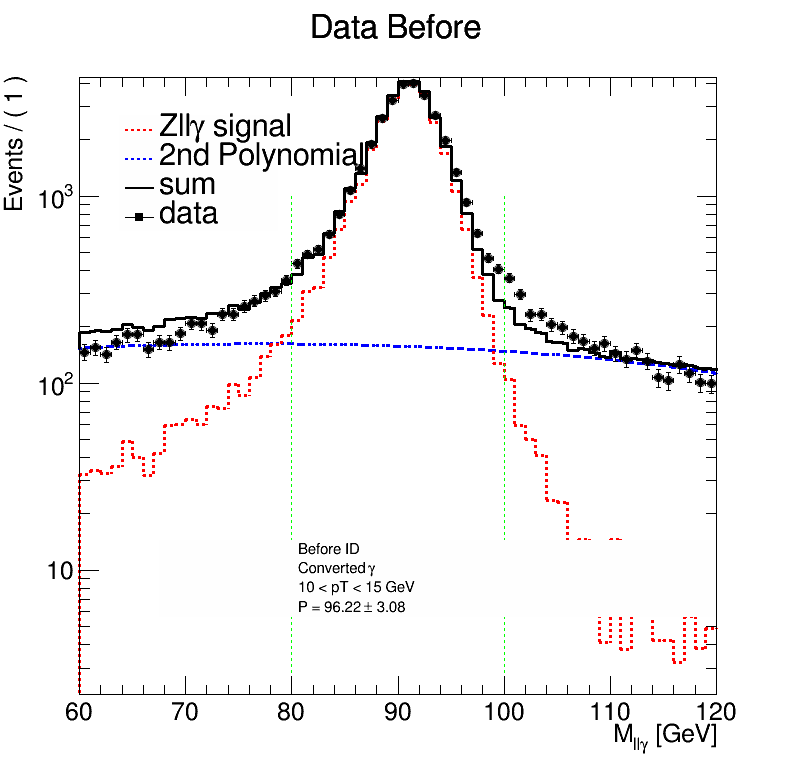
\includegraphics[width=.35\textwidth]{Adx/Adx2/Img/Convertedllg_Before_ID_Bin_0.png}}
	\subfloat[][]{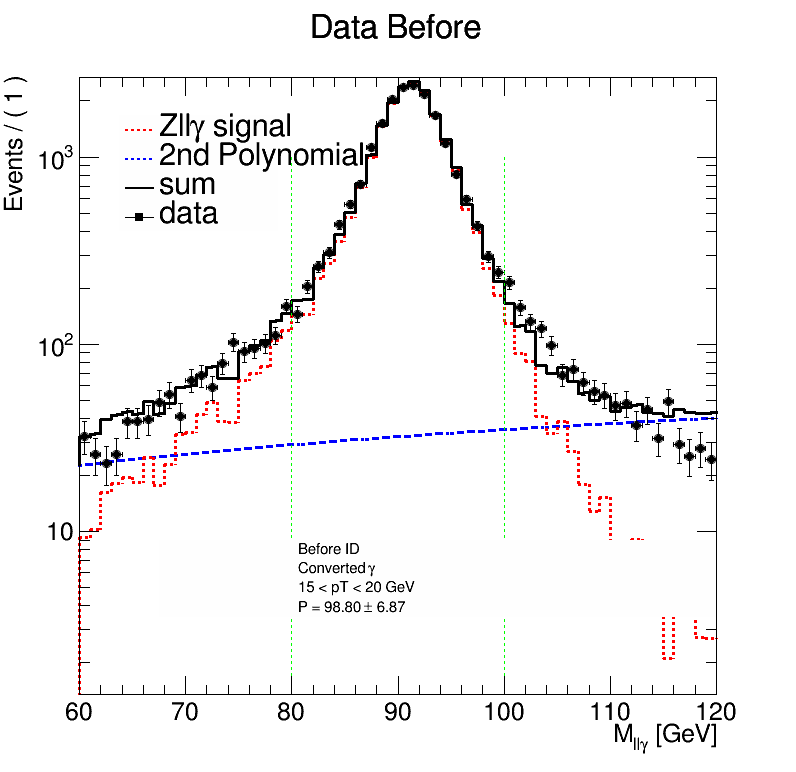
\includegraphics[width=.35\textwidth]{Adx/Adx2/Img/Convertedllg_Before_ID_Bin_1.png}} \\
	\subfloat[][]{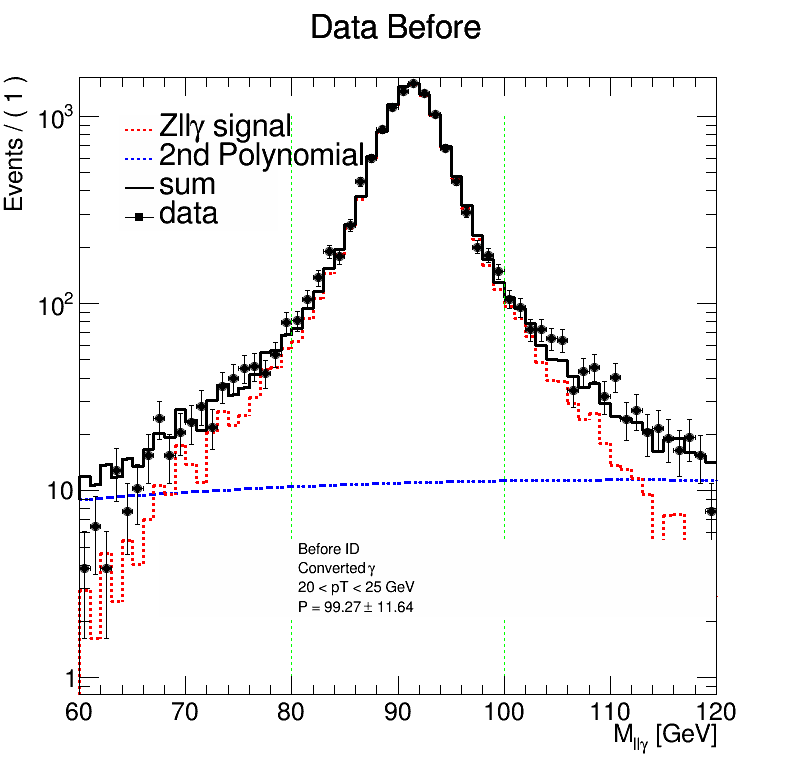
\includegraphics[width=.35\textwidth]{Adx/Adx2/Img/Convertedllg_Before_ID_Bin_2.png}}  
	\subfloat[][]{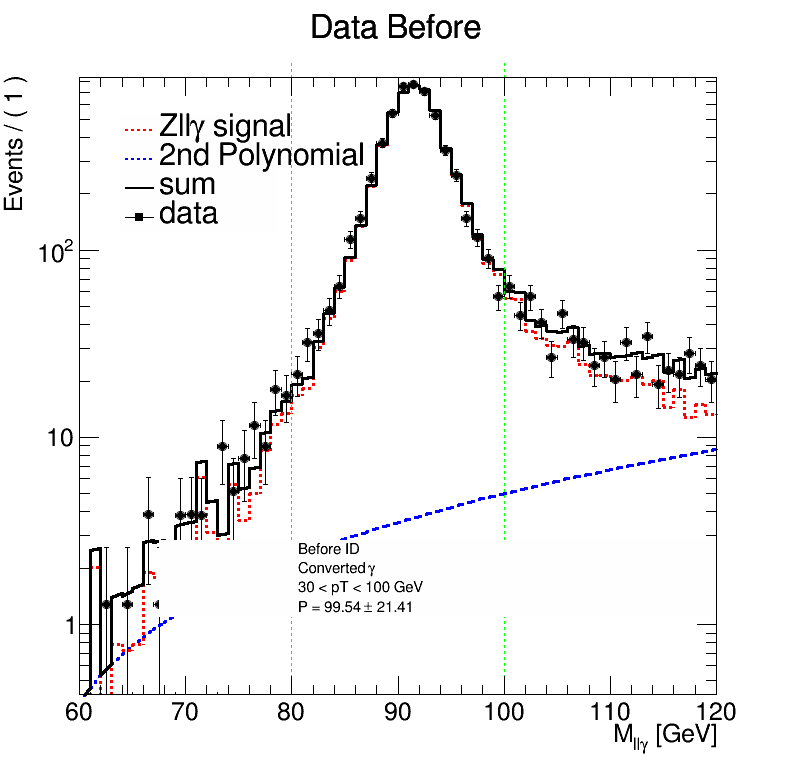
\includegraphics[width=.35\textwidth]{Adx/Adx2/Img/Convertedllg_Before_ID_Bin_4.png}}  
    \caption{Invariant mass ($m_{ll\gamma}$) distribution of events selected before Tight ID in data (black dots). The solid black line represents the fitting result of the data distribution with the sum of the signal (red dashed line) and the background (blue dashed line). The photons are reconstructed as converted.}
    \label{Eff:TemplateFit:C:Before}
\end{figure}

\begin{figure}[ht]
    \centering
	\subfloat[][]{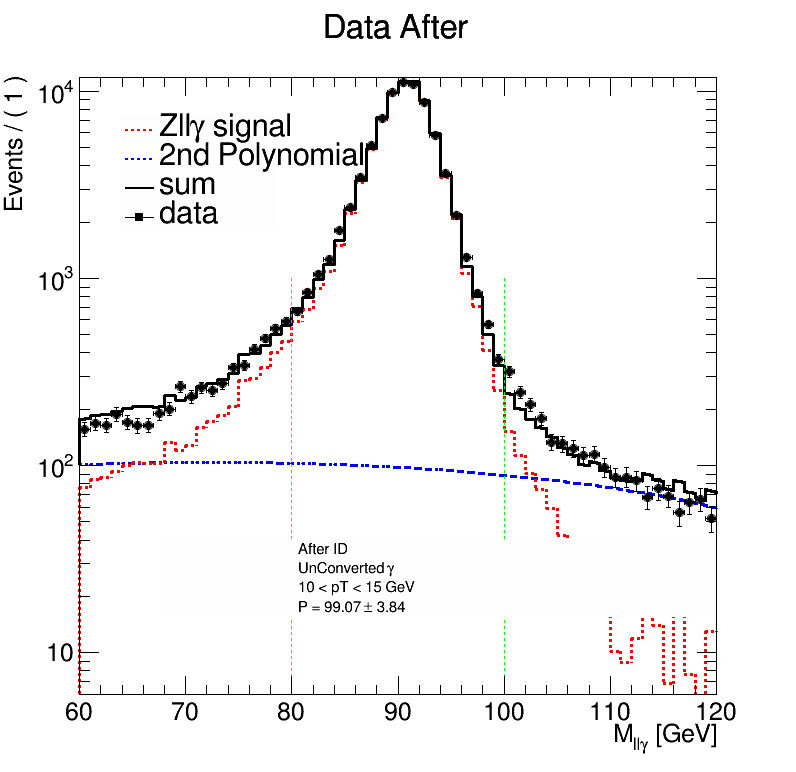
\includegraphics[width=.35\textwidth]{Adx/Adx2/Img/UnConvertedllg_After_ID_Bin_0.png}}
	\subfloat[][]{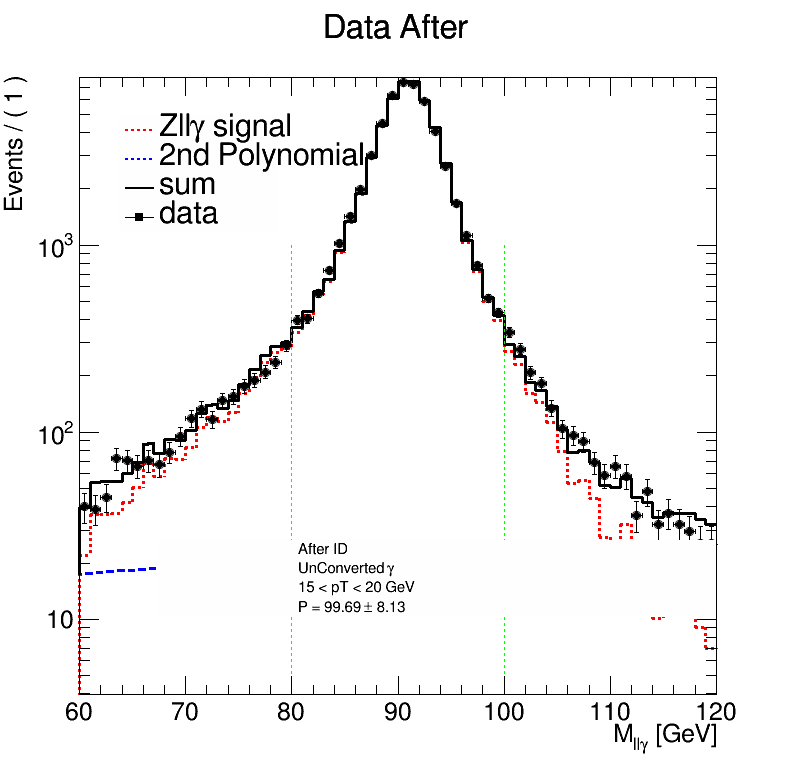
\includegraphics[width=.35\textwidth]{Adx/Adx2/Img/UnConvertedllg_After_ID_Bin_1.png}} \\
	\subfloat[][]{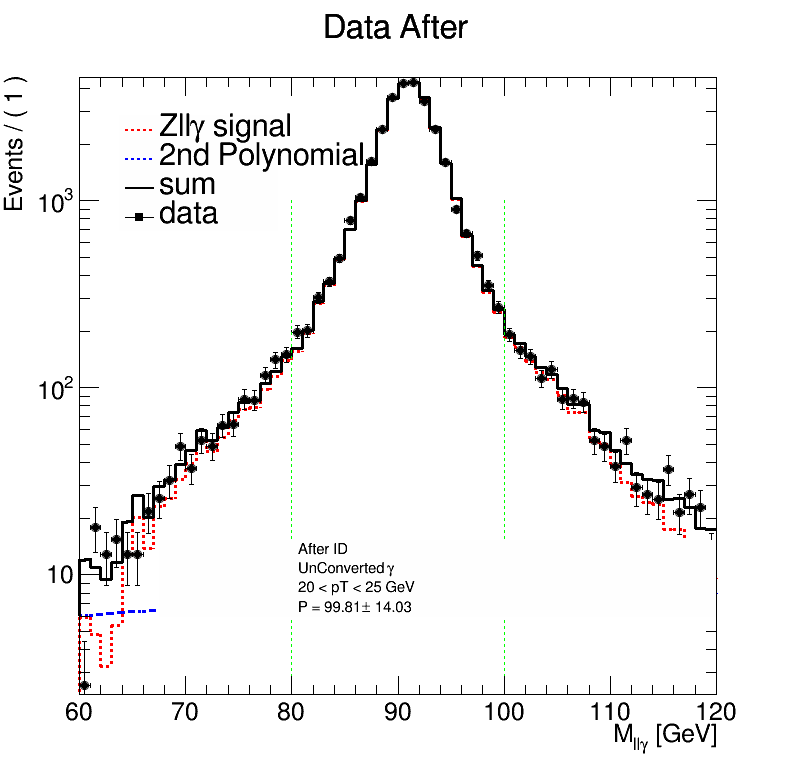
\includegraphics[width=.35\textwidth]{Adx/Adx2/Img/UnConvertedllg_After_ID_Bin_2.png}}  
	\subfloat[][]{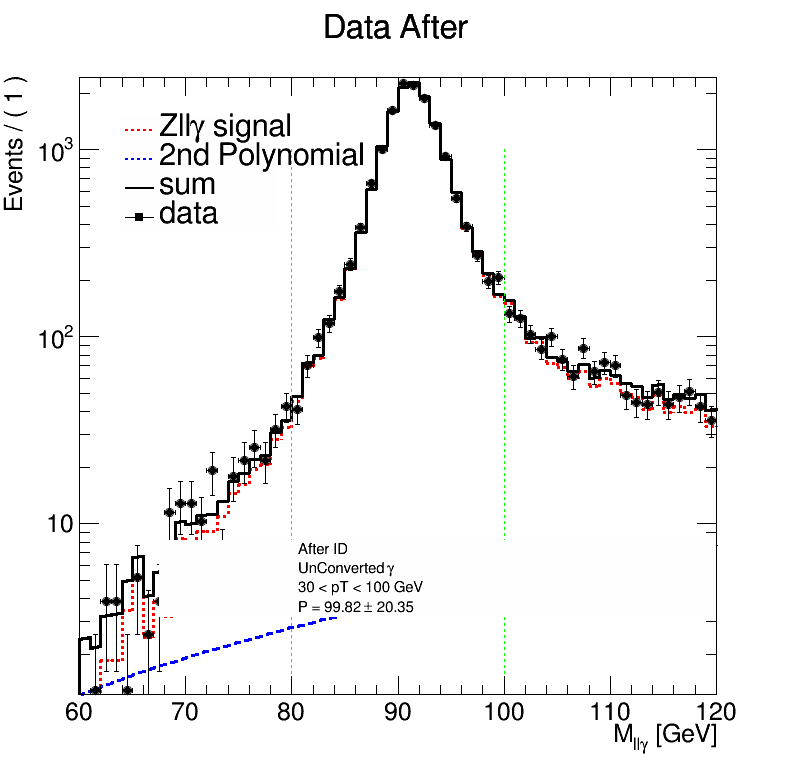
\includegraphics[width=.35\textwidth]{Adx/Adx2/Img/UnConvertedllg_After_ID_Bin_4.png}}  
    \caption{Invariant mass ($m_{ll\gamma}$) distribution of events selected after Tight ID in data (black dots). The solid black line represents the fitting result of the data distribution with the sum of the signal (red dashed line) and the background (blue dashed line). The photons are reconstructed as unconverted.}
    \label{Eff:TemplateFit:UnC:After}
\end{figure}

\begin{figure}[ht]
    \centering
	\subfloat[][]{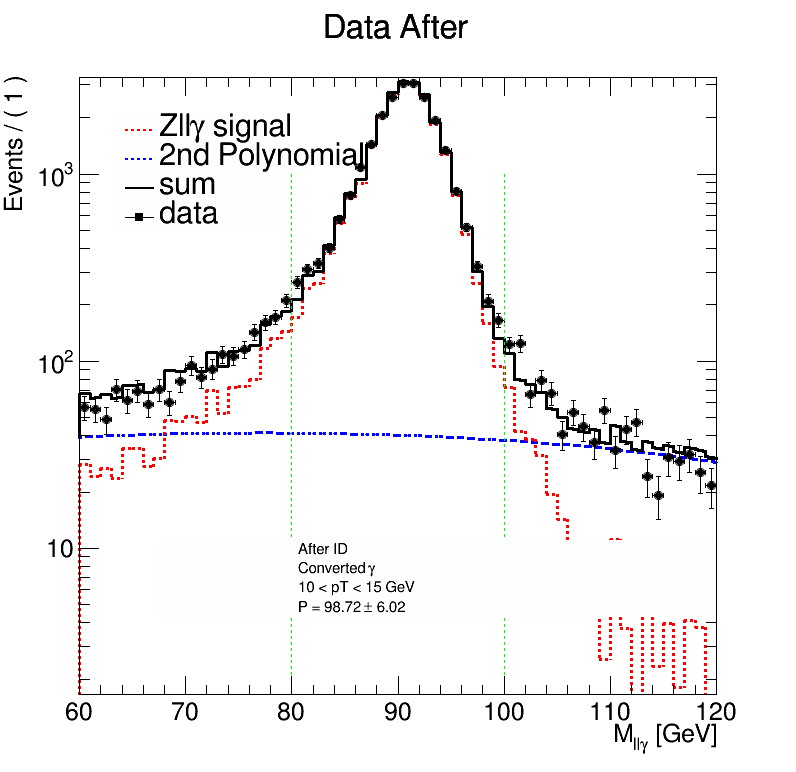
\includegraphics[width=.35\textwidth]{Adx/Adx2/Img/Convertedllg_After_ID_Bin_0.png}}
	\subfloat[][]{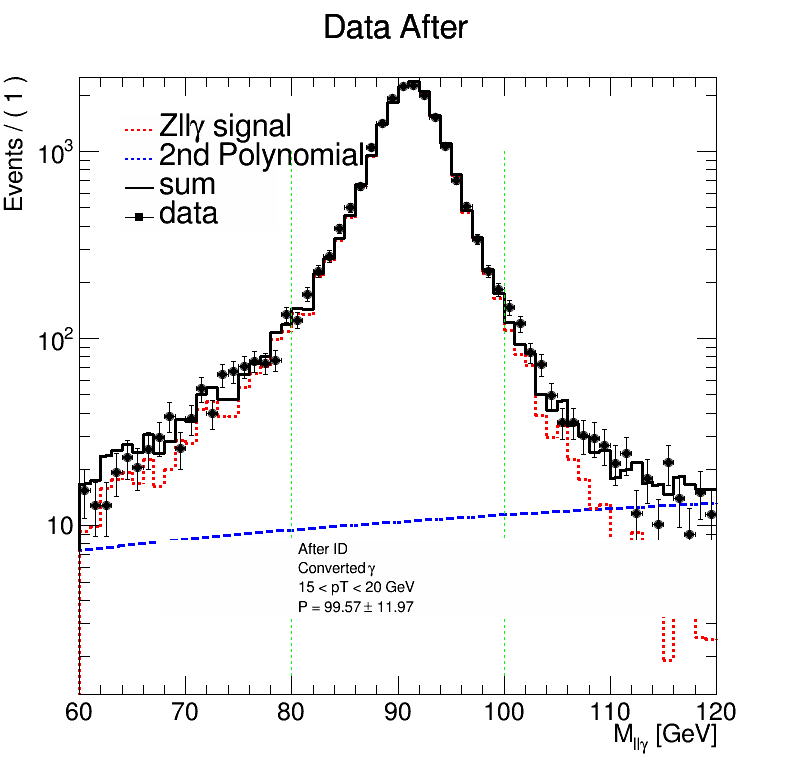
\includegraphics[width=.35\textwidth]{Adx/Adx2/Img/Convertedllg_After_ID_Bin_1.png}} \\
	\subfloat[][]{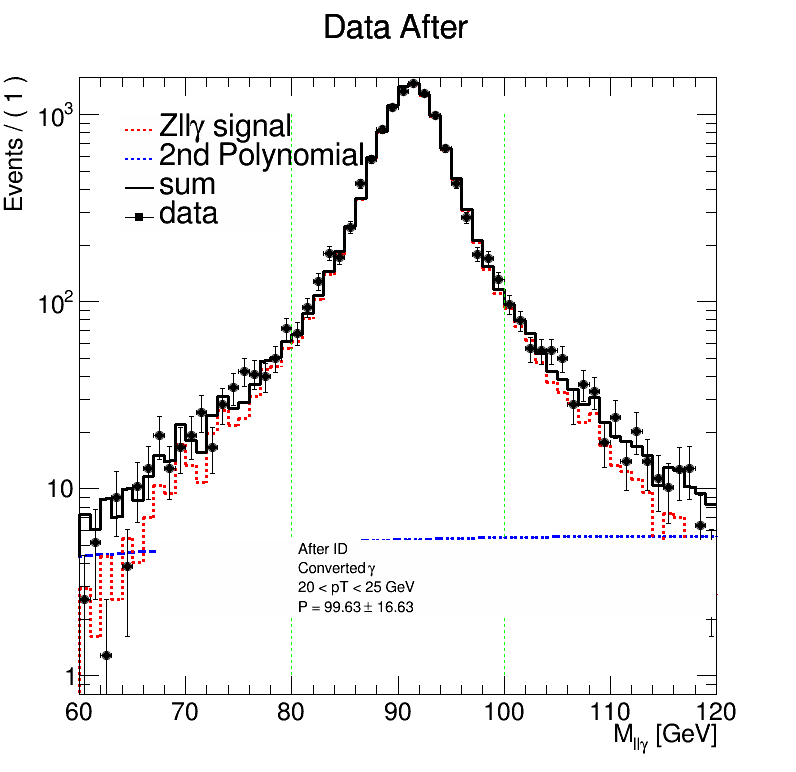
\includegraphics[width=.35\textwidth]{Adx/Adx2/Img/Convertedllg_After_ID_Bin_2.png}}  
	\subfloat[][]{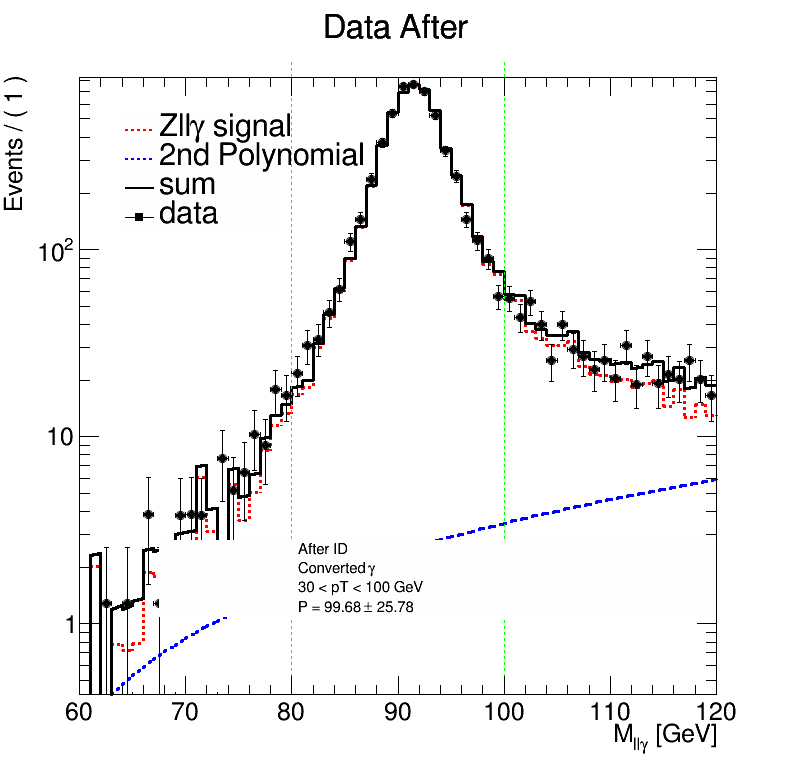
\includegraphics[width=.35\textwidth]{Adx/Adx2/Img/Convertedllg_After_ID_Bin_4.png}}  
    \caption{Invariant mass ($m_{ll\gamma}$) distribution of events selected after Tight ID in data (black dots). The solid black line represents the fitting result of the data distribution with the sum of the signal (red dashed line) and the background (blue dashed line). The photons are reconstructed as converted.}
    \label{Eff:TemplateFit:C:After}
\end{figure}

